\chapter{Umsetzung}

\section{Aktueller Stand der LSY}
\begin{figure}[h]
	\centering 
	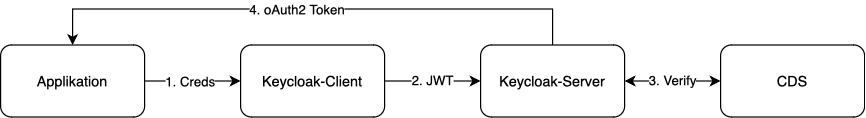
\includegraphics[width=1\textwidth]{img/abbildungen/Unknown.png}
	\captionsetup{format=hang}
	\caption{Aktuelle Umsetzung der Abteilung}
\end{figure}

\begin{itemize}
    \item Innerhalb der Abteilung wird eine passwortbasierte Authentifizierung durchgeführt, welche zusätzlich durch \ac{MFA} geschützt wird.
    \item Webanwendung nutzt einen eigene Anwendung, welche sich als Keycloak-Client aussgibt. Der Nutzer gibt seine Zugangsdaten an den Keycloak-Client weiter, welche diese verarbeitet. Dieser wandelt die Zugangsdaten in einen validen JWT-Token um und übergibt diesen an den Keycloak-Server. Dieser validiert die Zugangsdaten gegen die \ac{CDS}. Ist die Validierung erfolgreich, wird vom Keycloak-Server ein oAuth2-Token erstellt und zurück an die Applikation übergeben.
    \item Innerhalb der \ac{LSY} können sich Applikationen allerdings auch gegen das Azure \ac{AD} authentifizieren lassen. 
\end{itemize}

\section{Integration eines Yubikeys in die LSY}

\begin{figure}[h]
	\centering 
	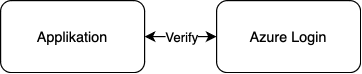
\includegraphics[width=0.6\textwidth]{img/abbildungen/azure_umsetzung.png}
	\captionsetup{format=hang}
	\caption{Umsetzungsmöglichkeit mit Azure \ac{AD}}
\end{figure}

\begin{itemize}
    \item Grundsätzlich gibt es zwei Möglichkeiten in die aktuelle Applikation eine passwortlose Authentifizierung mit Hilfe eines Yubikeys zu integrieren: Die Nutzung der Authentifizierung gegen das Azure \ac{AD} oder die eine veränderte Nutzung der aktuellen Keycloak-Lösung.

\end{itemize}

Eine Lufthansa-weite Policy für die Nutzung der Azure \ac{AD} verbietet allerdings die Nutzung eines Security Keys für eine \ac{SFA}. Hier kann der Security Key lediglich als zweiter Faktor genutzt werden. Dies kann jeder Nutzer selber verwalten. Registriert ein Nutzer seinen Security Key in seinem Profil, erscheint bei der Anmeldung (nach der Eingabe des Passwortes) ein zusätzliches Feld:

\begin{figure}[h]
	\centering 
	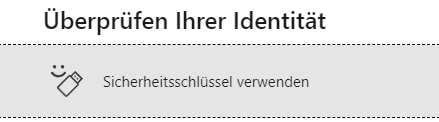
\includegraphics[width=0.6\textwidth]{img/abbildungen/azure_seckey.png}
	\captionsetup{format=hang}
	\caption{Umsetzungsmöglichkeit mit Keycloak}
\end{figure}

Verwendet der Nutzer einen Security Key wird dieser im Folenden aufgefordert die zugehörige PIN einzugeben und den Knopf des Security Keys zu drücken. Grundsätzlich ist eine passwortlose Authentifizierung mit Hilfe eines Security Keys innerhalb der Azure \ac{AD} möglich. Da eine Änderung dieser Lufthansa Policy notwendig wäre, übersteigt dies allerdings den Rahmen dieser Arbeit.

Da allerdings aktuell eine beschriebene Nutzung von Keycloak stattfindet und Keycloak eine passwortlose Authentifizierung mit Hilfe eines Security Keys unterstützt, wäre eine Umsetzung mit Hilfe von Keycloak möglich. Hierbei wird die aktuelle Lösung verändert und entsprechend angepasst:

\begin{figure}[h]
	\centering 
	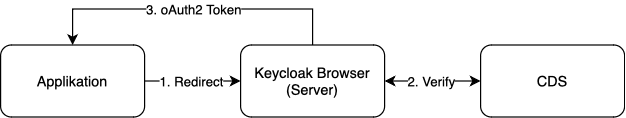
\includegraphics[width=1\textwidth]{img/abbildungen/keycloak_browser.png}
	\captionsetup{format=hang}
	\caption{Veränderter Keycloak-Login}
\end{figure}

Statt bei einer Anmeldung einen Client zu simulieren bietet Keycloak die Möglichkeit eine Anmeldung über eine Nutzeroberfläche zu realisieren. Dafür wird ein redirect auf die Keycloak-Login-Seite durchgeführt. Bei einer erfolgreichen Verifizierung wird der Nutzer zurück auf die Applikation geleitet und vom Keycloak-Server mit Hilfe eines oAuth2-Tokens authentifiziert. 

Um eine Passwortlose Authentifizierung in Keycloak zu ermöglichen, muss der Authentication Flow für eine Browser-Anmeldung modifiziert werden. Der angepasste Authentication Flow besteht aus folgenden Schritten:

\begin{figure}[h]
	\centering 
	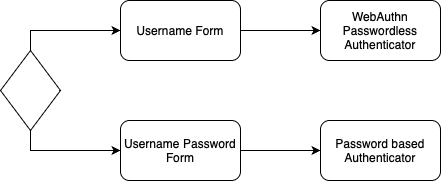
\includegraphics[width=0.7\textwidth]{img/abbildungen/authentication_flow.png}
	\captionsetup{format=hang}
	\caption{Authentication Flow}
\end{figure}

Hierbei wird die untere Hälfte der Grafik weiterhin ermöglicht, da es sich lediglich um einen Test handelt. Grundsätzlich wird diese nicht ermöglicht, da Keycloak eine reine passwortlose \ac{SFA} unterstützt.

Die obere Hälfte der Grafik entspricht dem für diese Arbeit relevanten Authentication Flow. Dabei wird der User zunächst aufgefordert seinen Nutzernamen einzugeben und anschließend seinen Security Key zu verwenden. Dies ist notwendig, um die Nutzung eines Security Keys für mehrere Zugänge zu ermöglichen. Ermöglicht man lediglich die Nutzung eines Zugangs pro Security Key, so wird die Eingabe des Nutzernamens nicht benötigt. Zusätzlich erfolgt eine Konfiguration des Keycloak-Servers, welche die Registrierung eines Security Keys bei der Registrierung eines neuen Nutzers ermöglicht.

Mit Hilfe dieser Konfiguration werden zwei Abläufe ermöglicht. Eine neue Registrierung:

\begin{figure}[H]
	\centering 
	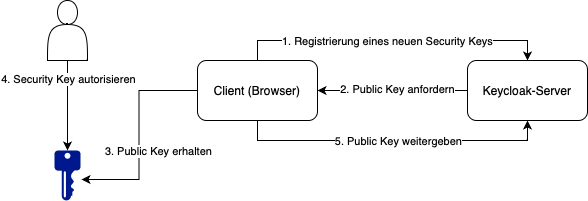
\includegraphics[width=1\textwidth]{img/abbildungen/register_simplified.png}
	\captionsetup{format=hang}
	\caption{Registrierung (vereinfacht)}
\end{figure}

Sowie eine neue Anmeldung:

\begin{figure}[H]
	\centering 
	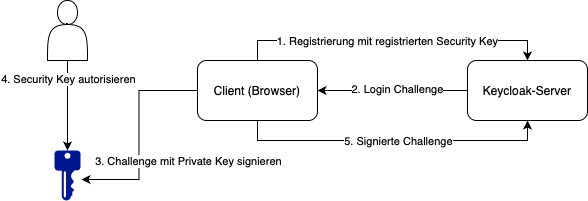
\includegraphics[width=1\textwidth]{img/abbildungen/login_simplified.png}
	\captionsetup{format=hang}
	\caption{Anmeldung (vereinfacht)}
\end{figure}

Die Grafiken stellen den vereinfachten Ablauf der Registrierung und Anmeldung mit Hilfe eines Security Keys dar. Die detailierte Darstellung der Funktionsweise ist in Kapitel 2.7 zu finden. Der entscheidende Unterschied der beiden Prozesse ist allerdings, dass bei der Registrierung lediglich der öffentliche Schlüssel übergeben wird, während bei der Anmeldung der private Schlüssel benötigt wird. Dieser wird allerdings nicht übergeben, sondern signiert eine Login Challenge, welche vom Keycloak-Server generiert wird. Kann der Keycloak-Server die Signatur mit Hilfe des gespeicherten öffentlichen Schlüssels verifizieren, wird der Nutzer authentifiziert. Sowohl die Registrierung als auch die Anmeldung erfolgen hierbei also nicht über die Anwendung selbst, sondern über den Keycloak-Server und dessen Nutzeroberfläche.

\section{User Feedback}
\begin{itemize}
    \item Fragebogen:
    \item How old are you?
    \item What is your role within the team?
    \item Wie zufrieden bist du mit der registrierung? (1-5)
    \item Wie zufrieden bist du mit der Anmeldung? (1-5)
    \item Findest du die passkey variante besser als einen yubikey?
    \item Have you ever used a security key before? Yes, and I still do - Yes, but I stopped using it - No - I don't know
    \item If Yes in which context? (private - work - both)
    \item Do you currently use a password manager at work? (Yes, I use it all/most of the time - Yes, but I only use it sometimes - No)
    \item Do you know how the Fido2 protocol works? (Yes - No - I don't know)
    \item Would you pay for a security key (about 50€)? (Yes - No - I don't know)
    \item Do you think security keys are more secure than passwords? (Yes - No - I don't know)
    \item Comments:
\end{itemize}

\section{Wirtschaftlichkeit}

\section{Nutzung des passwortlosen Verfahrens im privaten Kontext}